\documentclass[14pt]{extbook}
\usepackage{multicol, enumerate, enumitem, hyperref, color, soul, setspace, parskip, fancyhdr} %General Packages
\usepackage{amssymb, amsthm, amsmath, latexsym, units, mathtools} %Math Packages
\everymath{\displaystyle} %All math in Display Style
% Packages with additional options
\usepackage[headsep=0.5cm,headheight=12pt, left=1 in,right= 1 in,top= 1 in,bottom= 1 in]{geometry}
\usepackage[usenames,dvipsnames]{xcolor}
\usepackage{dashrule}  % Package to use the command below to create lines between items
\newcommand{\litem}[1]{\item#1\hspace*{-1cm}\rule{\textwidth}{0.4pt}}
\pagestyle{fancy}
\lhead{Progress Quiz 4}
\chead{}
\rhead{Version C}
\lfoot{5346-5907}
\cfoot{}
\rfoot{Summer C 2021}
\begin{document}

\begin{enumerate}
\litem{
Construct the lowest-degree polynomial given the zeros below. Then, choose the intervals that contain the coefficients of the polynomial in the form $ax^3+bx^2+cx+d$.\[ \frac{7}{3}, 1, \text{ and } \frac{-7}{2} \]\begin{enumerate}[label=\Alph*.]
\item \( a \in [0, 14], b \in [28, 31.1], c \in [12, 15], \text{ and } d \in [-57, -44] \)
\item \( a \in [0, 14], b \in [0.9, 2], c \in [-60, -55], \text{ and } d \in [-57, -44] \)
\item \( a \in [0, 14], b \in [0.9, 2], c \in [-60, -55], \text{ and } d \in [48, 54] \)
\item \( a \in [0, 14], b \in [40.6, 41.8], c \in [82, 89], \text{ and } d \in [48, 54] \)
\item \( a \in [0, 14], b \in [-4.2, 0.2], c \in [-60, -55], \text{ and } d \in [-57, -44] \)

\end{enumerate} }
\litem{
Describe the zero behavior of the zero $x = -4$ of the polynomial below.\[ f(x) = -4(x + 4)^{5}(x - 4)^{8}(x - 9)^{3}(x + 9)^{4} \]\begin{enumerate}[label=\Alph*.]
\begin{multicols}{2}\item 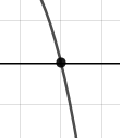
\includegraphics[width = 0.3\textwidth]{../Figures/polyZeroBehaviorAC.png}\item 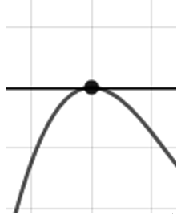
\includegraphics[width = 0.3\textwidth]{../Figures/polyZeroBehaviorBC.png}\item 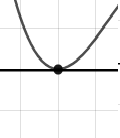
\includegraphics[width = 0.3\textwidth]{../Figures/polyZeroBehaviorCC.png}\item 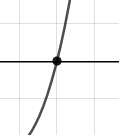
\includegraphics[width = 0.3\textwidth]{../Figures/polyZeroBehaviorDC.png}\end{multicols}\item None of the above.
\end{enumerate} }
\litem{
Construct the lowest-degree polynomial given the zeros below. Then, choose the intervals that contain the coefficients of the polynomial in the form $x^3+bx^2+cx+d$.\[ 5 - 2 i \text{ and } 1 \]\begin{enumerate}[label=\Alph*.]
\item \( b \in [-14, -9], c \in [37, 44], \text{ and } d \in [-34, -23] \)
\item \( b \in [2, 13], c \in [37, 44], \text{ and } d \in [27, 33] \)
\item \( b \in [-2, 6], c \in [-2, 5], \text{ and } d \in [-6, 1] \)
\item \( b \in [-2, 6], c \in [-6, -5], \text{ and } d \in [0, 8] \)
\item \( \text{None of the above.} \)

\end{enumerate} }
\litem{
Which of the following equations \textit{could} be of the graph presented below?
\begin{center}
    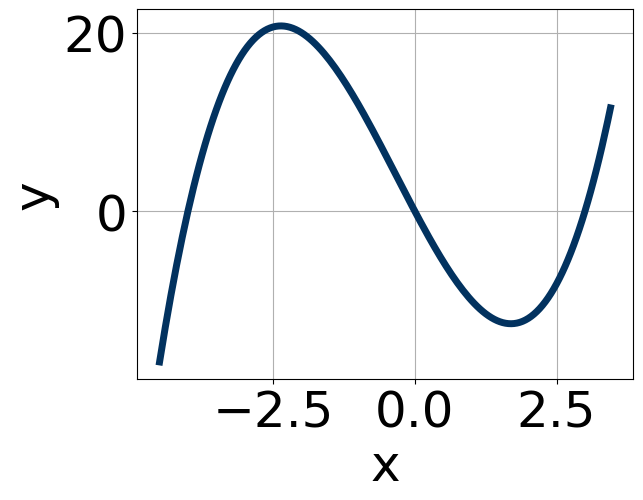
\includegraphics[width=0.5\textwidth]{../Figures/polyGraphToFunctionCopyC.png}
\end{center}
\begin{enumerate}[label=\Alph*.]
\item \( -11x^{6} (x + 4)^{11} (x - 3)^{5} \)
\item \( 7x^{9} (x + 4)^{11} (x - 3)^{9} \)
\item \( -6x^{7} (x + 4)^{5} (x - 3)^{5} \)
\item \( 6x^{8} (x + 4)^{4} (x - 3)^{11} \)
\item \( 8x^{8} (x + 4)^{5} (x - 3)^{7} \)

\end{enumerate} }
\litem{
Describe the zero behavior of the zero $x = -8$ of the polynomial below.\[ f(x) = 4(x - 7)^{5}(x + 7)^{3}(x + 8)^{9}(x - 8)^{8} \]\begin{enumerate}[label=\Alph*.]
\begin{multicols}{2}\item 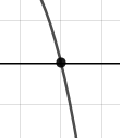
\includegraphics[width = 0.3\textwidth]{../Figures/polyZeroBehaviorCopyAC.png}\item 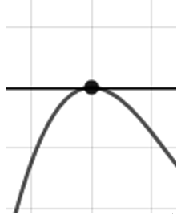
\includegraphics[width = 0.3\textwidth]{../Figures/polyZeroBehaviorCopyBC.png}\item 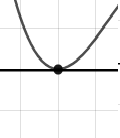
\includegraphics[width = 0.3\textwidth]{../Figures/polyZeroBehaviorCopyCC.png}\item 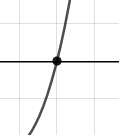
\includegraphics[width = 0.3\textwidth]{../Figures/polyZeroBehaviorCopyDC.png}\end{multicols}\item None of the above.
\end{enumerate} }
\litem{
Which of the following equations \textit{could} be of the graph presented below?
\begin{center}
    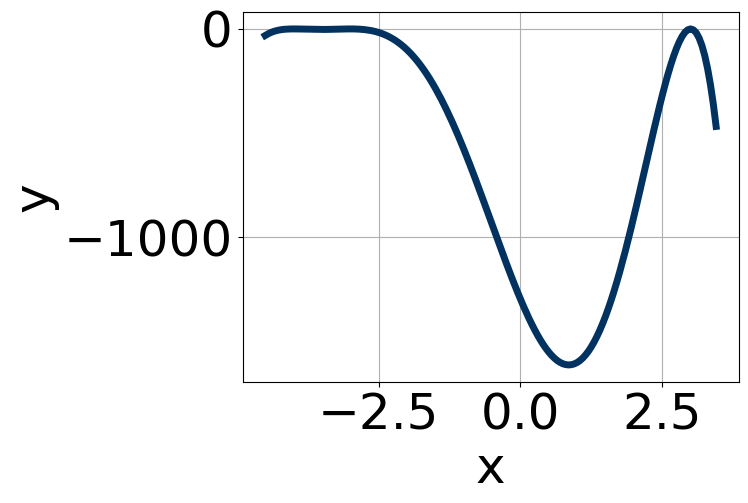
\includegraphics[width=0.5\textwidth]{../Figures/polyGraphToFunctionC.png}
\end{center}
\begin{enumerate}[label=\Alph*.]
\item \( 16(x + 4)^{10} (x - 3)^{10} (x + 3)^{6} \)
\item \( -4(x + 4)^{4} (x - 3)^{10} (x + 3)^{4} \)
\item \( 14(x + 4)^{10} (x - 3)^{4} (x + 3)^{11} \)
\item \( -7(x + 4)^{4} (x - 3)^{11} (x + 3)^{7} \)
\item \( -10(x + 4)^{10} (x - 3)^{6} (x + 3)^{11} \)

\end{enumerate} }
\litem{
Construct the lowest-degree polynomial given the zeros below. Then, choose the intervals that contain the coefficients of the polynomial in the form $x^3+bx^2+cx+d$.\[ 5 - 2 i \text{ and } 4 \]\begin{enumerate}[label=\Alph*.]
\item \( b \in [-17, -13], c \in [69, 79], \text{ and } d \in [-116, -115] \)
\item \( b \in [-7, 5], c \in [-5, 6], \text{ and } d \in [-9, -2] \)
\item \( b \in [-7, 5], c \in [-13, -6], \text{ and } d \in [10, 27] \)
\item \( b \in [14, 16], c \in [69, 79], \text{ and } d \in [114, 119] \)
\item \( \text{None of the above.} \)

\end{enumerate} }
\litem{
Describe the end behavior of the polynomial below.\[ f(x) = -9(x + 2)^{4}(x - 2)^{5}(x - 6)^{5}(x + 6)^{7} \]\begin{enumerate}[label=\Alph*.]
\begin{multicols}{2}\item 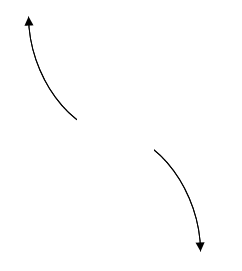
\includegraphics[width = 0.3\textwidth]{../Figures/polyEndBehaviorCopyAC.png}\item 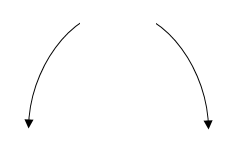
\includegraphics[width = 0.3\textwidth]{../Figures/polyEndBehaviorCopyBC.png}\item 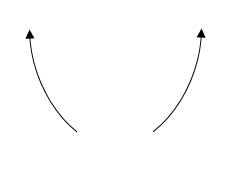
\includegraphics[width = 0.3\textwidth]{../Figures/polyEndBehaviorCopyCC.png}\item 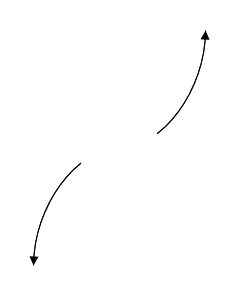
\includegraphics[width = 0.3\textwidth]{../Figures/polyEndBehaviorCopyDC.png}\end{multicols}\item None of the above.
\end{enumerate} }
\litem{
Describe the end behavior of the polynomial below.\[ f(x) = 9(x + 3)^{2}(x - 3)^{3}(x - 4)^{4}(x + 4)^{5} \]\begin{enumerate}[label=\Alph*.]
\begin{multicols}{2}\item 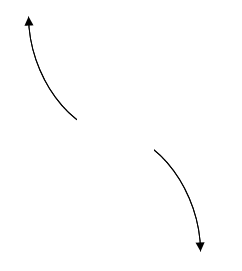
\includegraphics[width = 0.3\textwidth]{../Figures/polyEndBehaviorAC.png}\item 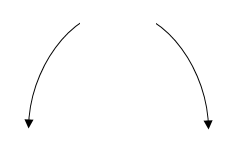
\includegraphics[width = 0.3\textwidth]{../Figures/polyEndBehaviorBC.png}\item 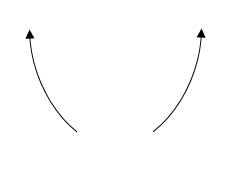
\includegraphics[width = 0.3\textwidth]{../Figures/polyEndBehaviorCC.png}\item 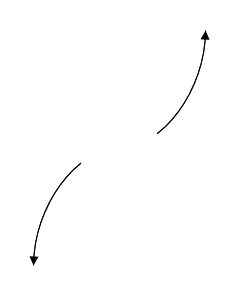
\includegraphics[width = 0.3\textwidth]{../Figures/polyEndBehaviorDC.png}\end{multicols}\item None of the above.
\end{enumerate} }
\litem{
Construct the lowest-degree polynomial given the zeros below. Then, choose the intervals that contain the coefficients of the polynomial in the form $ax^3+bx^2+cx+d$.\[ \frac{-7}{4}, \frac{-7}{5}, \text{ and } 4 \]\begin{enumerate}[label=\Alph*.]
\item \( a \in [20, 23], b \in [-144, -139], c \in [301, 307], \text{ and } d \in [-196, -195] \)
\item \( a \in [20, 23], b \in [9, 18], c \in [-207, -199], \text{ and } d \in [189, 200] \)
\item \( a \in [20, 23], b \in [-19, -15], c \in [-207, -199], \text{ and } d \in [-196, -195] \)
\item \( a \in [20, 23], b \in [-92, -78], c \in [-26, -20], \text{ and } d \in [189, 200] \)
\item \( a \in [20, 23], b \in [-19, -15], c \in [-207, -199], \text{ and } d \in [189, 200] \)

\end{enumerate} }
\end{enumerate}

\end{document}